% Define block styles
\tikzstyle{decision} = [diamond, draw, fill=blue!20, 
    text width=4.5em, text badly centered, inner sep=0pt]
\tikzstyle{block} = [rectangle, draw, fill=blue!20, 
    text width=5em, text centered, rounded corners, minimum height=4em]
\tikzstyle{line} = [draw, -latex']
\tikzstyle{cloud} = [draw, ellipse,fill=red!20, node distance=3cm,
    minimum height=2em]

%The two heuristical approaches

Apart from the implementation of the AMPL model we have also created two separate solvers of the problem using heuristics. One method was decided to be based on creating a pool of all week appearances that exists. Each week appearance contains a unique set of tasks during all seven days. After creating the pool of blocks these are assigned to the workers based on costs, one for each week. The other method ...
\begin{center}
	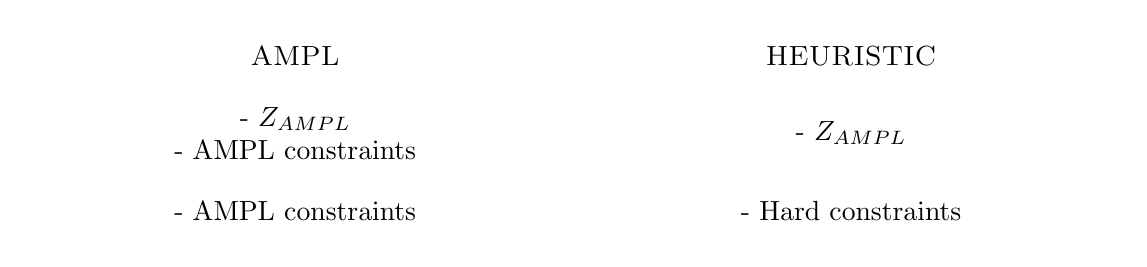
\begin{tikzpicture}[auto,
	block_center/.style ={rectangle, draw=black, thick, fill=white,
      text width=8em, text centered, minimum height=4em},
    block_left/.style ={rectangle, draw=black, thick, fill=white,
      text width=8em, text ragged, text centered, minimum height=4em, inner sep=6pt},
    block_noborder/.style ={rectangle, draw=none, thick, fill=none,
      text width=18em, text centered, minimum height=1em},
    block_assign/.style ={rectangle, draw=black, thick, fill=white,
      text width=18em, text ragged, minimum height=3em, inner sep=6pt},
    block_lost/.style ={rectangle, draw=black, thick, fill=white,
      text width=16em, text ragged, minimum height=3em, inner sep=6pt},
      line/.style ={draw, thick, -latex', shorten >=0pt}]
     \matrix [column sep=5mm,row sep=3mm] {
            % enrollment - Row 1
            \node [block_noborder] (AMPL) {\textsc{AMPL}}; 
			 & \node [block_noborder] (Heuristic) {\textsc{HEURISTIC}}; \\
			 % Row 2
			 \node [block_noborder] (ObjfunA) {- $Z_{AMPL}$ \\
			 - AMPL constraints};
			 & \node[block_noborder] (ObjfunH) {- $Z_{AMPL}$}; \\
			  % Row 3
			 \node [block_noborder] (ObjfunA) {- AMPL constraints};
			  & \node[block_noborder] (ObjfunH) {- Hard constraints}; \\
     };% end matrix
	\end{tikzpicture}
\end{center}

\section{Weekly scheduling approach} \label{Weekly}
In Appendix \ref{appendix:flow_charts}, Figure \ref{flow_chart}, is a flow chart of the implemented heuristic presented.

For every worker their information such as availability and qualification is inserted into a table template in Excel. It is then written to a text file using Visual Basic code, which in turn is read by the heuristic.



\subsection{Block creation} \label{block_creation}
A big part of this heuristic is to create the big pool of unique week appearances. These are then filtered for each of the worker based on its availability. The workers availability are generalized into three categories: \textit{Weekend week}, \textit{weekrest week} and \textit{weekday week}, where weekday week occurs three times during a five week period, see Table \ref{tab:Bob_avail}. 


One week block contains seven days and up to four shifts where each shift can contain up to three task types. Table \ref{Generalized weekblock} below is a representation of a general week block with all possible tasks for each day \textit{d} and shift \textit{s}. \textit{I} in the table represents "No task" is assigned that day, \textit{D} represents "Desk task" meaning either Exp or Info, \textit{PL} represents "Fetch list" and \textit{HB} represents "Hageby". 

\begin{table}[!h]
\centering
\caption{A generalized weekblock with all existing tasks}
\label{Generalized weekblock}
\begin{tabular}{cccccccc}
                         & Mon                         & Tue                         & Wed                         & Thu                         & Fri                         & Sat                         & Sun                         \\ \cline{2-8} 
\multicolumn{1}{c|}{08:00-10:00} & \multicolumn{1}{c|}{I,D,PL} & \multicolumn{1}{c|}{I,D,PL} & \multicolumn{1}{c|}{I,D,PL} & \multicolumn{1}{c|}{I,D,PL} & \multicolumn{1}{c|}{I,D,PL} & \multicolumn{1}{c|}{I,D,HB} & \multicolumn{1}{c|}{I,D,HB} \\ \cline{2-8} 
\multicolumn{1}{c|}{10:00-13:00} & \multicolumn{1}{c|}{D}      & \multicolumn{1}{c|}{D}      & \multicolumn{1}{c|}{D}      & \multicolumn{1}{c|}{D}      & \multicolumn{1}{c|}{D}      &       \\ \cline{2-6} 
\multicolumn{1}{c|}{13:00-16:00} & \multicolumn{1}{c|}{D}      & \multicolumn{1}{c|}{D}      & \multicolumn{1}{c|}{D}      & \multicolumn{1}{c|}{D}      & \multicolumn{1}{c|}{D}      &       \\ \cline{2-6} 
\multicolumn{1}{c|}{16:00-20:00} & \multicolumn{1}{c|}{D}      & \multicolumn{1}{c|}{D}      & \multicolumn{1}{c|}{D}      & \multicolumn{1}{c|}{D}      & \multicolumn{1}{c|}{D}      &       \\ \cline{2-6} 
\end{tabular}
\end{table}

Every day must contain exactly \textit{one} task from either of the four shifts when creating a week block. The tasks \textit{I} and \textit{PL} are ranging more than one shift. The duration of a PL is three shift and I refers to the entire day. Hence, they are both placed in the first shift to simplify the complete task representation. When creating the combinations of block appearances there are additional conditions that have to be met. These are:
\begin{enumerate}  
\item At most two tasks can be assigned the same shift and week.\label{first_item}
\item No more than two evenings are allowed each week, one of which is required to be a Friday. \label{second_item}
\item At most one PL is allowed in a weekblock. \label{third_item}
\item Saturday and Sunday shall always contain the same task type.\label{fourth_item}
\item If Saturday and Sunday contain Desk tasks, then so shall Friday afternoon (fourth shift). \label{friday_as_weekend}
\item No more than four tasks are allowed during the weekdays leaving at least one day without tasks. \label{fifth_item}
\end{enumerate}

%23,328 -> 9072 when item 4 applied
Too see the growth of the problem when more tasks are added, consider the following example: If item \ref{first_item}, \ref{second_item}, \ref{third_item}, \ref{friday_as_weekend} and \ref{fifth_item} are disregarded there exists $6^5*3 = 23,328$ unique weekblocks. In contrast, if Exp and Info were to be considered separately, instead of the combination of the two, the possible combinations would be $10^5*4 = 400,000$.  By applying all conditions the total amount of unique block appearances for this implementation are 4,175. 

An illustration of one of the 4,175 existing block can be seen in Table \ref{block_example} below.
\begin{table}[!h]
\centering
\caption{Illustration of one of the unique block appearances}
\label{block_example}
\begin{tabular}{cccccccc}
                           & Mon                                            & Tue                                             & Wed                    & Thu                                            & Fri                    & Sat                                             & Sun                                             \\ \cline{2-8} 
\multicolumn{1}{c|}{08:00-10:00}  & \multicolumn{1}{c|}{}                          & \multicolumn{1}{c|}{\cellcolor[HTML]{FCFF2F}PL} & \multicolumn{1}{c|}{I} & \multicolumn{1}{c|}{}                          & \multicolumn{1}{c|}{I} & \multicolumn{1}{c|}{\cellcolor[HTML]{FCFF2F}HB} & \multicolumn{1}{c|}{\cellcolor[HTML]{FCFF2F}HB} \\ \cline{2-8} 
\multicolumn{1}{c|}{10:00-13:00} & \multicolumn{1}{c|}{}                          & \multicolumn{1}{c|}{\cellcolor[HTML]{FCFF2F}}   & \multicolumn{1}{c|}{}  & \multicolumn{1}{c|}{}                          & \multicolumn{1}{c|}{}  &                                                 &                                                 \\ \cline{2-6}
\multicolumn{1}{c|}{13:00-16:00} & \multicolumn{1}{c|}{}                          & \multicolumn{1}{c|}{\cellcolor[HTML]{FCFF2F}}   & \multicolumn{1}{c|}{}  & \multicolumn{1}{c|}{\cellcolor[HTML]{FCFF2F}D} & \multicolumn{1}{c|}{}  &                                                 &                                                 \\ \cline{2-6}
\multicolumn{1}{c|}{16:00-20:00} & \multicolumn{1}{c|}{\cellcolor[HTML]{FCFF2F}D} & \multicolumn{1}{c|}{}                           & \multicolumn{1}{c|}{}  & \multicolumn{1}{c|}{}                          & \multicolumn{1}{c|}{}  &                                                 &                                                 \\ \cline{2-6}
\end{tabular}
\end{table}

This block contains five tasks; two of them are weekend tasks and three are weekday tasks. Which week this block can be assigned to is dependent on the worker's rotation. Since Hageby is assigned to the weekblock one can conclude that only a librarian can have this block assigned to itself. Due to this fact, the Desk tasks can imply either Exp or Info desk work as librarians are qualified for both.


\subsection{Block percolation}
After creating all existing week combinations they are percolated to each of the workers based on their availability in each of the three categories mentioned in Section \ref{block_creation}. Table \ref{blocks_available_per_worker} in Appendix \ref{appendix:weekblock} shows the results after this percolation has been made for all workers.


All of the values in the table are a subset of the total amount of 4,175 blocks. Knowing the structure of the problem, one can deduce that the amount of available weekrest blocks are always less than or equal to the available weekday blocks, as it should be. The only difference between the two mentioned block categories is when a worker is free from work due to its weekrest. Therefore, using this information one can interpret that they are equal when the worker is never working weekends.
\begin{table}[!h]
\centering
\caption{Typical availability for a generalized worker. Yellow signifies that the worker is available. In parenthesis, the weekend shift hours.}
\label{typical_availability}
\begin{tabularx}{\textwidth}{|X|l|l|l|l|l|l|l|X|}
\hline
%-------------------------------------------------------------------
\textbf{Weekend week}& \colcell \textbf{Mon} & \colcell \textbf{Tue} & \colcell \textbf{Wed} & \colcell \textbf{Thu} & \colcell \textbf{Fri} & \colcell \textbf{Sat} & \colcell \textbf{Sun}
\\ \hline 
%%------------------------------------------------------------------- 
%\rowcolor{Gray} 
\colcell 08:00-10:00 (11:00-16:00) & \colcelltwo & \colcelltwo & \colcelltwo & \colcelltwo & \colcelltwo & \colcelltwo & \colcelltwo
\\ \hline 
%%-------------------------------------------------------------------
%\rowcolor{Gray} 
\colcell 10:00-13:00 & \colcelltwo & \colcelltwo & \colcelltwo & \colcelltwo & \colcelltwo &   & 
\\ \hline 
%%-------------------------------------------------------------------
%\rowcolor{Gray} 
\colcell 13:00-16:00 & \colcelltwo & \colcelltwo & \colcelltwo & \colcelltwo & \colcelltwo & &
\\ \hline 
%%-------------------------------------------------------------------
%\rowcolor{Gray} 
\colcell 16:00-20:00 & & & \colcelltwo & & \colcelltwo & &
\\ \hline 
%%-------------------------------------------------------------------
\end{tabularx}
\begin{tabularx}{\textwidth}{|X|l|l|l|l|l|l|l|X|}
\hline
%-------------------------------------------------------------------
\textbf{Weekrest week}& \colcell \textbf{Mon} & \colcell \textbf{Tue} & \colcell \textbf{Wed} & \colcell \textbf{Thu} & \colcell \textbf{Fri} & \colcell \textbf{Sat} & \colcell \textbf{Sun}
\\ \hline 
%%------------------------------------------------------------------- 
%\rowcolor{Gray} 
\colcell 08:00-10:00 (11:00-16:00) & \colcelltwo & \colcelltwo & \colcelltwo & & & & 
\\ \hline 
%%-------------------------------------------------------------------
%\rowcolor{Gray} 
\colcell 10:00-13:00 & \colcelltwo & \colcelltwo & \colcelltwo & & & & 
\\ \hline 
%%-------------------------------------------------------------------
%\rowcolor{Gray} 
\colcell 13:00-16:00 & \colcelltwo & \colcelltwo & \colcelltwo & & & &
\\ \hline 
%%-------------------------------------------------------------------
%\rowcolor{Gray} 
\colcell 16:00-20:00 & & & \colcelltwo & & & &
\\ \hline 
%%-------------------------------------------------------------------
\end{tabularx}
\begin{tabularx}{\textwidth}{|X|l|l|l|l|l|l|l|X|}
\hline
%-------------------------------------------------------------------
\textbf{Weekday week}& \colcell \textbf{Mon} & \colcell \textbf{Tue} & \colcell \textbf{Wed} & \colcell \textbf{Thu} & \colcell \textbf{Fri} & \colcell \textbf{Sat} & \colcell \textbf{Sun}
\\ \hline 
%%------------------------------------------------------------------- 
%\rowcolor{Gray} 
\colcell 08:00-10:00 (11:00-16:00) & \colcelltwo & \colcelltwo & \colcelltwo & \colcelltwo & \colcelltwo & & 
\\ \hline 
%%-------------------------------------------------------------------
%\rowcolor{Gray} 
\colcell 10:00-13:00 & \colcelltwo & \colcelltwo & \colcelltwo & \colcelltwo & \colcelltwo &   & 
\\ \hline 
%%-------------------------------------------------------------------
%\rowcolor{Gray} 
\colcell 13:00-16:00 & \colcelltwo & \colcelltwo & \colcelltwo & \colcelltwo & \colcelltwo & &
\\ \hline 
%%-------------------------------------------------------------------
%\rowcolor{Gray} 
\colcell 16:00-20:00 & & & \colcelltwo & & & &
\\ \hline 
%%-------------------------------------------------------------------
\end{tabularx}
\begin{tabularx}{\textwidth}{|X|l|l|l|l|l|l|l|X|}
\hline
%-------------------------------------------------------------------
\textbf{Weekday week}& \colcell \textbf{Mon} & \colcell \textbf{Tue} & \colcell \textbf{Wed} & \colcell \textbf{Thu} & \colcell \textbf{Fri} & \colcell \textbf{Sat} & \colcell \textbf{Sun}
\\ \hline 
%%------------------------------------------------------------------- 
%\rowcolor{Gray} 
\colcell 08:00-10:00 (11:00-16:00) & \colcelltwo & \colcelltwo & \colcelltwo & \colcelltwo & \colcelltwo & & 
\\ \hline 
%%-------------------------------------------------------------------
%\rowcolor{Gray} 
\colcell 10:00-13:00 & \colcelltwo & \colcelltwo & \colcelltwo & \colcelltwo & \colcelltwo &   & 
\\ \hline 
%%-------------------------------------------------------------------
%\rowcolor{Gray} 
\colcell 13:00-16:00 & \colcelltwo & \colcelltwo & \colcelltwo & \colcelltwo & \colcelltwo & &
\\ \hline 
%%-------------------------------------------------------------------
%\rowcolor{Gray} 
\colcell 16:00-20:00 & & & \colcelltwo & & & &
\\ \hline 
%%-------------------------------------------------------------------
\end{tabularx}
\begin{tabularx}{\textwidth}{|X|l|l|l|l|l|l|l|X|}
\hline
%-------------------------------------------------------------------
\textbf{Weekday week}& \colcell \textbf{Mon} & \colcell \textbf{Tue} & \colcell \textbf{Wed} & \colcell \textbf{Thu} & \colcell \textbf{Fri} & \colcell \textbf{Sat} & \colcell \textbf{Sun}
\\ \hline 
%%------------------------------------------------------------------- 
%\rowcolor{Gray} 
\colcell 08:00-10:00 (11:00-16:00) & \colcelltwo & \colcelltwo & \colcelltwo & \colcelltwo & \colcelltwo & & 
\\ \hline 
%%-------------------------------------------------------------------
%\rowcolor{Gray} 
\colcell 10:00-13:00 & \colcelltwo & \colcelltwo & \colcelltwo & \colcelltwo & \colcelltwo &   & 
\\ \hline 
%%-------------------------------------------------------------------
%\rowcolor{Gray} 
\colcell 13:00-16:00 & \colcelltwo & \colcelltwo & \colcelltwo & \colcelltwo & \colcelltwo & &
\\ \hline 
%%-------------------------------------------------------------------
%\rowcolor{Gray} 
\colcell 16:00-20:00 & & & \colcelltwo & & & &
\\ \hline 
%%-------------------------------------------------------------------
\end{tabularx}
\end{table} 

Looking at a generalized worker's availability shown in Table \ref{typical_availability} one might think that there shall be more weekend blocks available than weekday blocks as the availability, almost in all cases, are higher for weekend blocks. This is not the case as all blocks without weekend tasks are removed in the percolation. This means that all combinations with "No task" on weekends are removed, as well as the case that is shown in Table \ref{Friday_percolation}. The case in Table \ref{Friday_percolation} occurs when a worker is assigned weekend Desk tasks and therefore can not be assigned any other task that Friday.





\begin{table}[!h]
\centering
\caption{A weekend block with Desk tasks preventing any other tasks on Fridays.}
\label{Friday_percolation}
\begin{tabular}{cccccccc}
                                 & Mon                    & Tue                    & Wed                    & Thu                    & Fri                                            & Sat                                            & Sun                                            \\ \cline{2-8} 
\multicolumn{1}{c|}{08:00-10:00} & \multicolumn{1}{c|}{X} & \multicolumn{1}{c|}{X} & \multicolumn{1}{c|}{X} & \multicolumn{1}{c|}{X} & \multicolumn{1}{c|}{\cellcolor[HTML]{000000}}  & \multicolumn{1}{c|}{\cellcolor[HTML]{FCFF2F}D} & \multicolumn{1}{c|}{\cellcolor[HTML]{FCFF2F}D} \\ \cline{2-8} 
\multicolumn{1}{c|}{10:00-13:00} & \multicolumn{1}{c|}{}  & \multicolumn{1}{c|}{}  & \multicolumn{1}{c|}{}  & \multicolumn{1}{c|}{}  & \multicolumn{1}{c|}{\cellcolor[HTML]{000000}}  &                                                &                                                \\ \cline{2-6}
\multicolumn{1}{c|}{13:00-16:00} & \multicolumn{1}{c|}{}  & \multicolumn{1}{c|}{}  & \multicolumn{1}{c|}{}  & \multicolumn{1}{c|}{}  & \multicolumn{1}{c|}{\cellcolor[HTML]{000000}}  &                                                &                                                \\ \cline{2-6}
\multicolumn{1}{c|}{16:00-20:00} & \multicolumn{1}{c|}{}  & \multicolumn{1}{c|}{}  & \multicolumn{1}{c|}{}  & \multicolumn{1}{c|}{}  & \multicolumn{1}{c|}{\cellcolor[HTML]{FCFF2F}D} &                                                &                                                \\ \cline{2-6}
\end{tabular}
\end{table}

 "X" in Table \ref{Friday_percolation} can represent any task and shifts colored in black means that no other task can be assigned that shift.

\subsection{Rotation assignment} \label{rotation}
There are 35 weekend workers available of which 21 are librarians and 14 are assistants. The demand of weekend workers each week is seven, i.e. the demand for five weeks is exactly $7*5 = 35$ workers. Another requirement in excess to seven workers each weekend is that at least four of them have to be librarians due to three librarians are needed in Information desks and one in Hageby. Therefore, it deems reasonable to swap rotations between workers in the destroy so that it always remains feasible. 

A random generator is used in the assignment of rotations that always makes sure that the two mentioned requirements are met. Furthermore, all of the LoW-workers have fixed weekends and hence are not given new rotations in the destroy/repair loop and is more thoroughly described in Section \ref{LoW_assignment} below. 

Table \ref{rotation_assignment} shows a destroy/repair iteration regarding rotation assignments. The amount of workers being destroyed in each iteration is three.

\begin{table}[!h]
\centering
\caption{An iteration in the destroy/repair loop showing a swap of weekends when three workers are destroyed}
\label{rotation_assignment}
Initial assignment:\\
\begin{tabular}{l|llllll}
\rowcolor[HTML]{C0C0C0}
Week       & 1 & 2 & 3 & 4 & 5  \\ \hline
Librarians & 4 & 4 & 5 & 4 & 4  \\ \hline
Assistants & 3 & 3 & 2 & 3 & 3 
\end{tabular}\\
After destroy:\\
\begin{tabular}{l|llllll}
\rowcolor[HTML]{C0C0C0}
Week       & 1                         & 2                         & 3                         & 4                         & 5                          \\ \hline
Librarians & \cellcolor[HTML]{FFFE65}3 & 4 & \cellcolor[HTML]{FFFE65}4 & 4 & 4  \\ \hline
Assistants & 3 & \cellcolor[HTML]{FFFE65}2 & 2 & 3 & 3
\end{tabular}\\
After repair:\\
\begin{tabular}{l|llllll}
\rowcolor[HTML]{C0C0C0}
Week       & 1 & 2 & 3 & 4 & 5  \\ \hline
Librarians & \cellcolor[HTML]{9AFF99}4 & \cellcolor[HTML]{9AFF99}5 & 4 & 4 & 4  \\ \hline
Assistants & 3 & 2 & \cellcolor[HTML]{9AFF99}3 & 3 & 3 
\end{tabular}
\end{table}

Yellow indicates that a worker, either librarian or assistant, has been destroyed that week and green indicates that a worker has been repaired. Comparing the "Initial assignment" with "After repair" a swap can be seen between week 2 and 3. Worth noting is that a swap can occur even if the amount of qualified workers remains the same after a repair. To understand this, imagine that two librarians with different rotations are destroyed, then two cases can occur: Either they are assigned the same rotation as before or they swap weekends. 


\subsection{Assignment of Library on Wheels} \label{LoW_assignment}
In order to avoid creating enormous amounts of block combinations, LoW tasks are assigned manually. To assign LoW manually also lead to a fix weekend rotation for the five LoW-workers. This slightly reduces the degrees of freedom of the problem as the LoW-workers' rotation will remain unchanged. However, as there are only a couple different set of feasible LoW assignments it shall not be the deciding factor for the quality of the solution.

Without a manual assignment of LoW the number of existing tasks in a weekblock would increase significantly. The number of tasks would increase from 36 to 43, as there are seven LoW tasks during a week, resulting in a lot more than 4,175 unique week appearances. % %ändra sista

\subsection{Initial solution} \label{initial_solution}
The initial solution is created in a similar fashion as the repair function in this heuristic. Based on a greedy heuristic the best weekblock for a random worker and week is found and inserted. This is done until every worker have one weekend block, one weekrest block and three weekday blocks assigned to them.

To find the best weekblock several costs have been introduced to measure whether a block is good or bad to assign a worker. Say, if the library demands two librarians at the Information desk Monday at 08:00 and currently there are one assigned, then it would be good to assign another one. Such an assignment will, therefore, be rewarded using a cost. Good assignments will provide negative costs and bad assignments will provide positive costs to the objective function value.

Table \ref{block_to_evaluate} together with Figure \ref{flow_chart_cost} shows an increment where different cost parameters have to be considered when evaluating a block before assigning it to a worker. In order to calculate demand costs for the PL in the library, assume that this block which is being evaluated is to be inserted at week three.

% Please add the following required packages to your document preamble:
% \usepackage[table,xcdraw]{xcolor}
% If you use beamer only pass "xcolor=table" option, i.e. \documentclass[xcolor=table]{beamer}
\begin{table}[!h]
\centering
\caption{A block example to be evaluated using costs}
\label{block_to_evaluate}
\begin{tabular}{cccccccc}
                                 & Mon                                             & Tue                    & Wed                                            & Thu                    & Fri                                            & Sat                    & Sun                    \\ \cline{2-8} 
\multicolumn{1}{c|}{08:00-10:00} & \multicolumn{1}{c|}{\cellcolor[HTML]{FCFF2F}PL} & \multicolumn{1}{c|}{I} & \multicolumn{1}{c|}{}                          & \multicolumn{1}{c|}{I} & \multicolumn{1}{c|}{}                          & \multicolumn{1}{c|}{I} & \multicolumn{1}{c|}{I} \\ \cline{2-8} 
\multicolumn{1}{c|}{10:00-13:00} & \multicolumn{1}{c|}{\cellcolor[HTML]{FCFF2F}}   & \multicolumn{1}{c|}{}  & \multicolumn{1}{c|}{}                          & \multicolumn{1}{c|}{}  & \multicolumn{1}{c|}{\cellcolor[HTML]{FCFF2F}D} &                        &                        \\ \cline{2-6}
\multicolumn{1}{c|}{13:00-16:00} & \multicolumn{1}{c|}{\cellcolor[HTML]{FCFF2F}}   & \multicolumn{1}{c|}{}  & \multicolumn{1}{c|}{\cellcolor[HTML]{FCFF2F}D} & \multicolumn{1}{c|}{}  & \multicolumn{1}{c|}{}                          &                        &                        \\ \cline{2-6}
\multicolumn{1}{c|}{16:00-20:00} & \multicolumn{1}{c|}{}                           & \multicolumn{1}{c|}{}  & \multicolumn{1}{c|}{}                          & \multicolumn{1}{c|}{}  & \multicolumn{1}{c|}{}                          &                        &                        \\ \cline{2-6}
                                 &                                                 &                        &                                                &                        &                                                &                        &                        \\
\multicolumn{3}{c}{Task to be evaluated}                                                                    &                                                &                        &                                                &                        &                        \\
                                 & Mon                                             &                        &                                                &                        &                                                &                        &                        \\ \cline{2-2}
\multicolumn{1}{c|}{08:00-10:00} & \multicolumn{1}{c|}{\cellcolor[HTML]{FCFF2F}PL} &                        &                                                &                        &                                                &                        &                        \\ \cline{2-2}
\multicolumn{1}{c|}{10:00-13:00} & \multicolumn{1}{c|}{\cellcolor[HTML]{FCFF2F}}   &                        &                                                &                        &                                                &                        &                        \\ \cline{2-2}
\multicolumn{1}{c|}{13:00-16:00} & \multicolumn{1}{c|}{\cellcolor[HTML]{FCFF2F}}   &                        &                                                &                        &                                                &                        &                        \\ \cline{2-2}
\end{tabular}
\end{table}


% % FLOW CHART of COSTS
\begin{figure}[!h]
  \caption{A flow chart of appearing costs when a PL is assigned a block on a Monday, third week relative to the library schedule.}
  \centering
	\scalebox{0.85}{ \label{flow_chart_cost}
		\begin{tikzpicture}[node distance = 2cm, auto]
		    % Place nodes
		    \node [decision] (demand) {Need for another PL-worker Monday week 3?};
		    %Invisible node
		    \node[below of= demand, node distance=3.5cm,scale=0.01](inv){};
		    
		    \node [decision, left of= inv, node distance = 3.5cm] (whoami1) {Am I ass/lib?};
		    \node [decision, right of= inv, node distance = 3.5cm] (whoami2) {Am I ass/lib?};
		    
		    %Invisible nodes
		    \node[below of= whoami1, node distance=3cm,scale=0.01](inv2){};
		    \node[below of= whoami2, node distance=3cm,scale=0.01](inv3){};
		    
		    \node[block, left of= inv2] (add_ass_cost1) {Add positive assistant demand cost};
		    \node[block, right of= inv2] (add_lib_cost1) {Add positive librarian demand cost};
		    \node[block, left of= inv3] (add_ass_cost2) {Add negative assistant demand cost};
		    \node[block, right of= inv3] (add_lib_cost2) {Add negative librarian demand cost};
			\node[decision, below of= demand, node distance = 11cm] (too_many) {Have I too many PL already?};
			
			%Invisible node
			\node[below of= too_many, node distance=3cm,scale=0.01](inv4){};
			\node[block, left of= inv4, node distance=2cm] (pl_good) {Add negative PL amount cost};
			\node[block, right of= inv4, node distance=2cm] (pl_violate) {Add positive PL amount cost};
			
		    % Draw edges
		    \path [line] (demand) -- node[left]{no}(whoami1);
		    \path [line] (demand) -- node[right]{yes}(whoami2);
		    \path [line] (whoami1) -- node[left]{ass}(add_ass_cost1);
		    \path [line] (whoami1) -- node[right]{lib}(add_lib_cost1);
		    \path [line] (whoami2) -- node[left]{ass}(add_ass_cost2);
		    \path [line] (whoami2) -- node[right]{lib}(add_lib_cost2);
		    \path [line] (add_ass_cost1) -- (too_many.north);
		    \path [line] (add_lib_cost1) -- (too_many.north);
		    \path [line] (add_ass_cost2) -- (too_many.north);
		    \path [line] (add_lib_cost2) -- (too_many.north);
		    \path [line] (too_many) -- node[left]{no}(pl_good);
		    \path [line] (too_many) -- node[right]{yes}(pl_violate);
		    
		    %First cost
		    \draw [color=gray!70,thick](-8,-9) rectangle(8,2);
		    \node[draw] at (-6.5,1.5) {PL demand cost};
		    %Second cost
		    \draw [color=gray!70,thick](-4,-16.5) rectangle(4,-9);
   		    \node[draw] at (-2.5,-9.5) {PL amount cost};
		    
		\end{tikzpicture}
		}
\end{figure}

    


\subsection{Costs}
In order to find a feasible solution many of the implemented costs must be carefully chosen. Presently, there are 16 existing costs where some of them are correlated with each other. The solution behaves differently depending on the relation between the costs changes.

Six of the costs are presented in Figure \ref{flow_chart_cost}. They have all been assigned unique values so that, for example, positive assistant demand cost differs from negative assistant demand cost in absolute value. To explain why, one can imagine a case where four workers are demanded of which two have to be librarians, see Table \ref{library_solutions}. The first case, where one assistant and three librarians have been assigned, is more desirable than the case with three assistants and one librarian. In the first case it is still a feasible solution as the qualification of assistants are a subset of the librarians. The second case is feasible, however, not optimal due to the exceeding use of librarians. The optimal solution is shown in green as Case 3.

\begin{table}[!h]
\centering
\caption{Library demand at a shift and solution qualities.}
\label{library_solutions}
\begin{tabular}{|l|l|l|}
\hline
\rowcolor[HTML]{C0C0C0} 
Demand:                         & \multicolumn{2}{l|}{\cellcolor[HTML]{C0C0C0}4 workers ($\geq 2$ librarians)} \\ \hline
\rowcolor[HTML]{FD6864} 
\cellcolor[HTML]{C0C0C0}Case 1: & 3 assistants, 1 librarian                  & (infeasible)                 \\ \hline
\rowcolor[HTML]{FFFE65} 
\cellcolor[HTML]{C0C0C0}Case 2: & 1 assistant, 3 librarians                  & (feasible)                     \\ \hline
\rowcolor[HTML]{34FF34} 
\cellcolor[HTML]{C0C0C0}Case 3:  & 2 assistants, 2 librarians                 & (optimal)                      \\ \hline
\end{tabular}
\end{table}

The complete list of costs with description can be seen in Table \ref{tab:all_costs}. 

\begin{table}[!h]
\centering
\caption{List of all costs with description.}
\label{tab:all_costs}
\begin{tabular}{|l|l|}
\hline
\rowcolor[HTML]{C0C0C0} 
Cost name                                      & Description       \\ \hline
\rowcolor[HTML]{FD6864} 
\multicolumn{2}{|c|}{\cellcolor[HTML]{FD6864}Demand costs}    \\ \hline
Demand\_few\_assistants                        & In need of more assistants to fill quota.                  \\ \hline
Demand\_few\_librarians                        & In need of more librarians to fill quota.                 \\ \hline
Demand\_many\_assistants                       & More assistants assigned than needed (redundancy).           \\ \hline
Demand\_many\_librarians                       & More librarians assigned than reference value.                  \\ \hline
Demand\_few\_total                             & Incorrect amount of workers assigned a task.                  \\ \hline
Demand\_many\_total                            & Incorrect amount of workers assigned a task.                  \\ \hline
Demand\_evening\_cost         & Incorrect amount of workers assigned an evening task (more crucial).\\ \hline
Demand\_PL\_good\_assistant        & Assigning a PL to assistant, empty before assignment.            \\ \hline
Demand\_PL\_good\_librarian        & Assigning a PL to librarian, empty before assignment.           \\ \hline
Demand\_PL\_bad\_assistant         & Assigning a PL to assistant, others already assigned.           \\ \hline
Demand\_PL\_bad\_librarian         & Assigning a PL to librarian, others already assigned.             \\ \hline
\rowcolor[HTML]{FD6864} 
\multicolumn{2}{|c|}{\cellcolor[HTML]{FD6864}PL amount costs} \\ \hline
PL\_good\_amount                  & Assigning PL when in need of more for feasibility.                  \\ \hline
PL\_violate\_amount             & Assigning more PL than allowed to that worker.                  \\ \hline
\rowcolor[HTML]{FD6864} 
\multicolumn{2}{|c|}{\cellcolor[HTML]{FD6864}Weekend costs}   \\ \hline
HB\_amount                       & No or more than one HB workers assigned the same weekend.   \\ \hline
No\_weekend                &                   \\ \hline
\rowcolor[HTML]{FD6864} 
\multicolumn{2}{|c|}{\cellcolor[HTML]{FD6864}Stand-in costs}  \\ \hline
Stand\_in\_cost                     & Occuring when a possible stand-in is ruined due to assignment.    \\ \hline
\end{tabular}
\end{table}

\subsection{Destroy}
The destroy consists of two contiguous steps: Choosing three workers to destroy and then destroying their assigned blocks. The LoW tasks remain unchanged even if a worker assigned those tasks is destroyed. 
\subsection{Repair}
Initially in the repair function the destroyed workers are assigned new rotations, see Table \ref{rotation_assignment}, followed by five new week blocks. Which order the blocks are inserted in is randomly generated. For each iteration is one of the three workers randomly chosen followed by one block that has not been reassigned until all 15 destroyed weeks have been repaired. Which week block that is chosen is based on the costs listed in Table \ref{tab:all_costs}. 
\subsection{Evaluation of solution}
After each destroy/repair loop the new solution is evaluated. It is common for the new solution to be worse than the previous one. However, all new solutions are accepted regardless.

All costs are regarded in the evaluation function. If there are any demand differences in the library or any differences in amount of PL assigned to a worker these are given the respective costs. Furthermore, the amount of stand-ins is evaluated here provided with a negative cost showing that these are desired.

If there are no infeasibilities in the solution the evaluation function will return the value zero, unless there are stand-ins. In case there are stand-ins a negative value can be returned. 
\subsection{Final phase}
At the end of a run there are mostly a few infeasibilities left that do not get solved. To fix this, a final phase was implemented. Whenever a run is "relatively close" to a solution and it is "theoretically possible" to find a solution the final phase is initiated. "Relatively close" means in this case that the only infeasibility is the lack of workers at a handful of weekday shifts. "Theoretically possible" means that there are more stand-ins available all days where the infeasibility occurs.

The final phase destroys one random week for a random worker and immediately repairs it, resulting in the same or better solution until it is feasible. % %In discussion: Sometimes it does not find a feasible solution due to the worker had already four tasks assigned, i.e. the required block does not exist.

Due to well chosen cost parameter values the run will always eventually get relatively close and reach the final phase. If there are fewer stand-ins available a day where workers are lacking the solution will be discarded before entering the final phase. 
